\subsection{Signal Showdown: What's the Term for FM Interference?}

\begin{tcolorbox}[colback=gray!10, colframe=black, title=E4C03]
What is the term for the suppression in an FM receiver of one signal by another stronger signal on the same frequency?
\begin{enumerate}[label=\Alph*.]
    \item Desensitization
    \item Cross-modulation interference
    \item \textbf{Capture effect}
    \item Frequency discrimination
\end{enumerate} \end{tcolorbox}

\subsubsection{Related Concepts}

The phenomenon described in the question relates to how Frequency Modulation (FM) receivers handle signals received at the same frequency. Understanding the capture effect is essential for anyone studying radio communications, particularly in the context of analog broadcasting systems. 

1. \textbf{Desensitization:} This refers to a reduction in an FM receiver’s sensitivity due to the presence of another strong signal. This term typically describes a different scenario than what the question asks.

2. \textbf{Cross-modulation interference:} This describes a situation where two signals interact, causing the modulation of one signal to affect another. However, this is not the specific phenomenon where one signal suppresses the other.

3. \textbf{Capture effect:} This is the correct answer and describes how an FM receiver is capable of locking onto one signal if there are two signals present on the same frequency. The stronger signal will dominate, effectively suppressing the weaker signal, allowing the listener to only hear the stronger station.

4. \textbf{Frequency discrimination:} This refers to the ability of a receiver to distinguish between different frequencies or signals but does not specifically refer to the suppression of one signal by another.

\subsubsection{Calculation Step-by-Step}

While the question itself does not involve a direct calculation, it is essential to consider the following when analyzing signals:

- If we denote the power of the stronger signal as \( P_s \) and the power of the weaker signal as \( P_w \), the capture effect can be qualitatively described as the receiver favoring the signal with the higher \( P_s \).

- The criterion for capture might be expressed in terms of received signal-to-noise ratios. If the ratio between the two signals exceeds a certain threshold, the receiver tends to capture the stronger signal.

\subsubsection{Diagram}

To illustrate the concept of the capture effect, we can depict a simplified diagram of signal strength:

\begin{center}
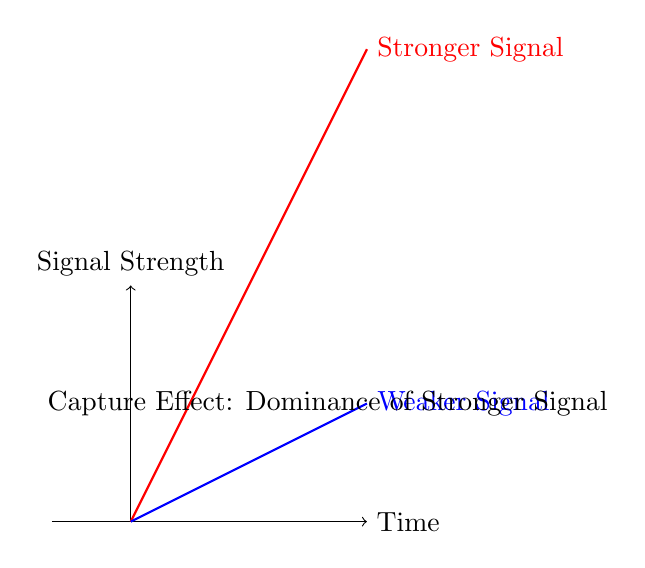
\begin{tikzpicture}
    \draw[->] (0,0) -- (0,3) node[above] {Signal Strength};
    \draw[->] (-1,0) -- (3,0) node[right] {Time};
    \draw[red, thick] plot[domain=0:3] (\x, {2*\x}) node[right] {Stronger Signal};
    \draw[blue, thick] plot[domain=0:3] (\x, {0.5*\x}) node[right] {Weaker Signal};

    \node at (2.5,1.5) {Capture Effect: Dominance of Stronger Signal};
\end{tikzpicture}
\end{center}
